\documentclass{article}
\usepackage[margin=0.5in]{geometry}\usepackage{tikz}
\begin{document}
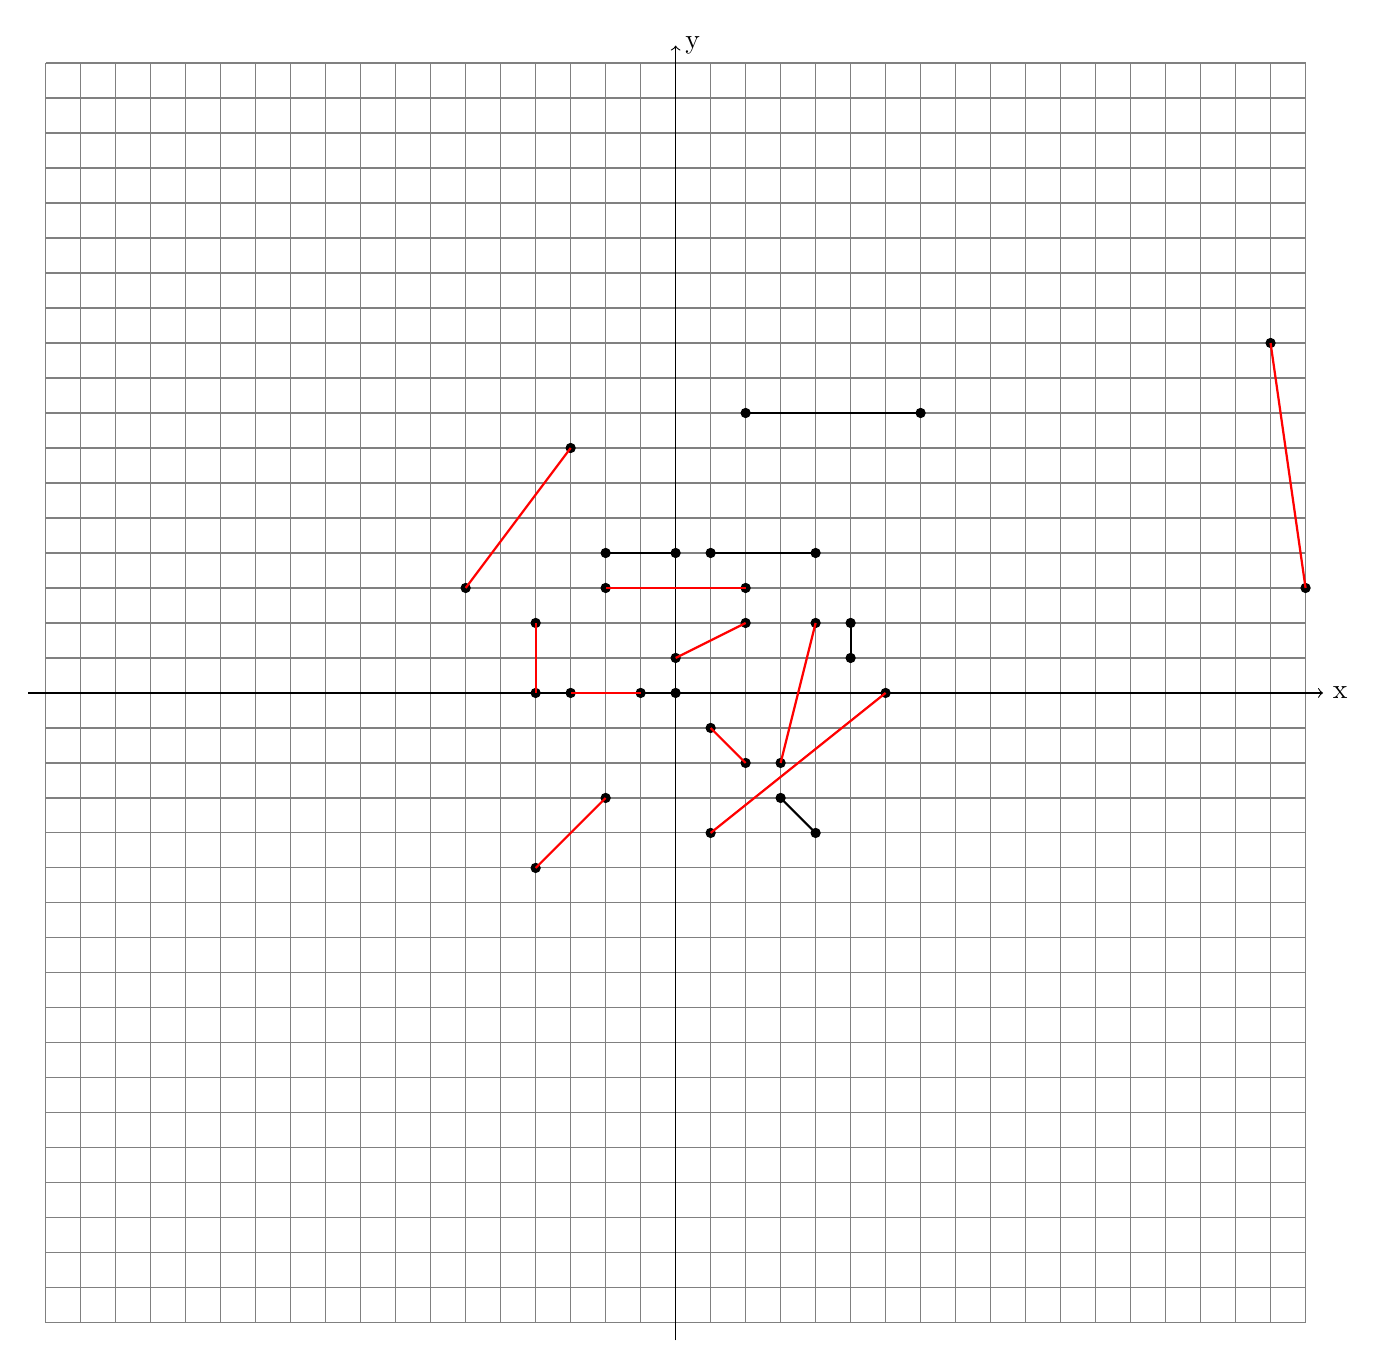
\begin{tikzpicture}[scale=0.444444] % <- Scale picture
   % Coordinate system grid
   \draw[step=1.0,gray,thin] (-18,-18) grid (18,18);
   % Coordinate system axis
   \draw[->] (-18.5,0) -- (18.5,0) node[right] {x};
   \draw[->] (0,-18.5) -- (0,18.5) node[right] {y};
   \draw [fill] (0,0) circle [radius=0.13];
   \draw [fill] (4,4) circle [radius=0.13];
   \draw [fill] (1,4) circle [radius=0.13];
   \draw [thick] (4,4) -- (1,4);
   \draw [fill] (2,3) circle [radius=0.13];
   \draw [fill] (-2,3) circle [radius=0.13];
   \draw [thick, red] (2,3) -- (-2,3);
   \draw [fill] (1,-4) circle [radius=0.13];
   \draw [fill] (6,0) circle [radius=0.13];
   \draw [thick, red] (1,-4) -- (6,0);
   \draw [fill] (-4,2) circle [radius=0.13];
   \draw [fill] (-4,0) circle [radius=0.13];
   \draw [thick, red] (-4,2) -- (-4,0);
   \draw [fill] (-4,-5) circle [radius=0.13];
   \draw [fill] (-2,-3) circle [radius=0.13];
   \draw [thick, red] (-4,-5) -- (-2,-3);
   \draw [fill] (3,-2) circle [radius=0.13];
   \draw [fill] (4,2) circle [radius=0.13];
   \draw [thick, red] (3,-2) -- (4,2);
   \draw [fill] (2,2) circle [radius=0.13];
   \draw [fill] (0,1) circle [radius=0.13];
   \draw [thick, red] (2,2) -- (0,1);
   \draw [fill] (0,4) circle [radius=0.13];
   \draw [fill] (-2,4) circle [radius=0.13];
   \draw [thick] (0,4) -- (-2,4);
   \draw [fill] (7,8) circle [radius=0.13];
   \draw [fill] (2,8) circle [radius=0.13];
   \draw [thick] (7,8) -- (2,8);
   \draw [fill] (18,3) circle [radius=0.13];
   \draw [fill] (17,10) circle [radius=0.13];
   \draw [thick, red] (18,3) -- (17,10);
   \draw [fill] (5,1) circle [radius=0.13];
   \draw [fill] (5,2) circle [radius=0.13];
   \draw [thick] (5,1) -- (5,2);
   \draw [fill] (1,-1) circle [radius=0.13];
   \draw [fill] (2,-2) circle [radius=0.13];
   \draw [thick, red] (1,-1) -- (2,-2);
   \draw [fill] (3,-3) circle [radius=0.13];
   \draw [fill] (4,-4) circle [radius=0.13];
   \draw [thick] (3,-3) -- (4,-4);
   \draw [fill] (-3,7) circle [radius=0.13];
   \draw [fill] (-6,3) circle [radius=0.13];
   \draw [thick, red] (-3,7) -- (-6,3);
   \draw [fill] (-1,0) circle [radius=0.13];
   \draw [fill] (-3,0) circle [radius=0.13];
   \draw [thick, red] (-1,0) -- (-3,0);
\end{tikzpicture}
\end{document}
